\documentclass[9pt]{report}
\usepackage{graphicx}
\usepackage[utf8]{inputenc}
%\usepackage[T1]{fontenc}
\usepackage{textcomp}
%\usepackage[dutch]{babel}
\usepackage{amsmath, amssymb}

\begin{document}
\title{Wald's General Relatvity \protect\\ Chapter 1 Problems}
\author{Anthony Steel}
\date{\today}
\maketitle
\begin{enumerate}
  \item \textbf{Car and Garage Paradox. The lack of a notion of absolute
      simultaneity in special relativity leads to many supposed paradoxes. One
      of the most famous of these involves a car and a garage of equal proper
      length. The driver speeds toward the garage, and a doorman at the garage
      is instructed to slam the door shut as soon as the back end of the car
      enters the garage. According to the doorman, "the car Lorentz contracted
      and easily fitted into the garage when I slammed the door". According to
      the driver, "the garage Lorentz contracted and was too small for the car
      when I entered the garage." Draw a spacetime diagram showing the above
      events and explain what really happens. Is the doorman's statement
      correct? For definiteness, assume that the car crashes through the
      back wall of the garage without stopping or slowing down.}

      The doorman's statement is correct but the doorman and
      driver disagree on the order of events. In the doorman's frame, he sees
      the end of the car coincident with him and closes the door. In his frame,
      the car is Lorentz contracted so that it has not broken through the wall yet.
      To be a nice guy, he decides to send a message to the driver telling them
      to stop the car so that the car does not break through the wall.

      \begin{figure}
        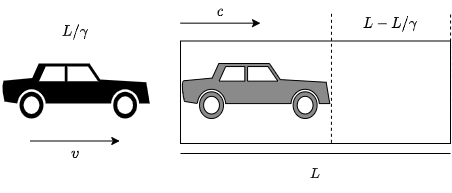
\includegraphics[width=0.95\textwidth]{images/carandgarageparadox.png}
        \caption{The car and garage paradox in the doorman's frame.}
        \label{doorman}
      \end{figure}

      Let $L$ be the proper length of the car and garage, $v$ be the velocity
      of the car in the doorman's reference frame, and $\gamma$ be the Lorentz
      factor.

      In the doorman's frame, he observes the car to be $L / \gamma$. When he
      closes the door, the car has not crashed through the end of the garage
      and the distance from the front of the car to the end of the garage is:
      \[
        \Delta L = L (1 - \frac{1}{\gamma})
      \]
      as shown in \ref{doorman}. Assume for simplicity that there is a detector
      at the end of the garage that will absorb the signal from the doorman. If
      the signal has been absorbed it is green and if not it is red. The driver
      simply observes the detector when he passes to see if he should stop or
      not.

      When the doorman emits the light signal to tell the driver to stop the car,
      the light takes a time:
      \[
        \Delta t_c = L / c
      \]
      to reach the end of the garage. The car however takes:
      \[
        \Delta t_v = \frac{\Delta L}{v} = \frac{L}{v} ( 1 - \frac{1}{\gamma}})
      \]
      If $\Delta t_c \leq \Delta t_v $ the car stops but if $\Delta t_c > \Delta t_v$
      the car crashes through the end of the garage. Assume:
      \[
        \begin{align}
          \Delta t_c  &> \Delta t_v \\
          \frac{L}{c} &> \frac{L}{v} ( 1 - \frac{1}{\gamma}) \\
          \frac{v}{c} &> ( 1 - \frac{1}{\gamma}) \\
          \frac{v}{c} &> ( 1 - \sqrt{1 - \frac{v^2}{c^2}} ) \\
          \sqrt{1 - \frac{v^2}{c^2}} &> 1 - \frac{v}{c}\\
          \sqrt{(1 - \frac{v}{c})(1 + \frac{v}{c})} &> 1 - \frac{v}{c} \\
          \sqrt{1 + \frac{v}{c}} &> \sqrt{1 - \frac{v}{c}}
       \end{align}
      \]
      This is always true, so the car always crashes through the end of the garage
      before the doorman can tell the driver to stop. This resolves the apparent
      paradox.

      However, it is clear that the order of events is not the same. As mentioned
      in the problem definition, the driver sees the garage Lorentz contracted
      so he crashes through the garage and then observes the door close. In
      the doorman's frame the order of events is inverted.

      \begin{figure}
        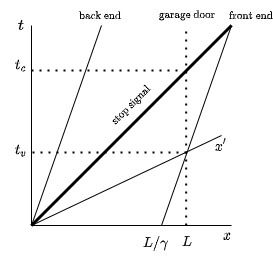
\includegraphics[width=0.70\textwidth]{images/carandgarage_spacetime.png}
        \caption{Minkowski diagram in the reference frame of the doorman}
        \label{spacetime}
      \end{figure}
      In hindsight, this is obvious from constructing a correct Minkowski
      diagram as shown in \ref{spacetime}.
  \end{enumerate}
\end{document}
